
% 和文概要
\begin{abstract}
JavaScriptとAndroid NFCで実世界GUIを実現できるフレームワーク GoldFishを実装した。GoldFishを使うことで、Android端末で実世界の物に触れることで操作対象を指定し、ユーザーやコンテキスト、ジェスチャー入力を認識して操作するアプリケーションを簡単に実装する事ができる。
\end{abstract}

% 英文概要
\begin{eabstract}
GoldFish is Real-world GUI Framework. It enables to develop Android application which detects the target object, user, context and gesture input using simple JavaScript and Android NFC.
\end{eabstract}

\maketitle

% 本文ここから
\section{実世界GUI}\label{sec:Introduction}
本研究の目的は、実世界GUI\cite{実世界GUI}を日常的に使えるようにする事である。実世界GUIは、コンピュータのグラフィカルユーザインタフェース(GUI)に似たしくみを実世界で使うという概念である。

塚田らのUbi-Finger\cite{Ubi-Finger}は、対象を指さす事で選択し、ジェスチャーで操作するための手袋型装置を開発した。また暦本は複数のコンピュータ間でマウスのドラッグアンドドロップの様にデータをやりとりする手法\cite{pick-and-drop}を提案した。椎尾らは、マウスとバーコードリーダーを一体化させることであらゆる物に対してマウスで操作できるようにした。\cite{field-mouse}

GUIには、コンピュータの画面上にゴミ箱や窓などの現実世界のメタファーを提示してユーザーに理解しやすくしている部分と、データを扱うためにドロップダウンメニューやスクロールバーなどのディスプレイならではの新しいユーザインタフェースとが組み合わさってできている。我々の生活にはたくさんのコンピュータが埋め込まれているが、電子錠つきの自動ドアをキーパッドで操作して開けていたり、ラップトップPCから目の前にあるプリンターに印刷させるのに画面上でプリンタの名前を指定して送信していたりと、操作と効果の対応づけがわかりにくく効率が悪い事がある。そうではなくむしろ、実世界でもGUIのようにメタファーによるインタフェースとデータ操作用インタフェースが混在している方が使い勝手が良いのではないかと考えた。

既存の実世界GUIの研究から、1.対象の指定 2.ジェスチャーやGUIによる操作 3.ユーザーとコンテキストの判別 4.他のシステムとの通信 の4つの要素が重要であると考えられる。これらを利用するアプリケーションを簡単に実装でき、また日常的に使えるような仕組みを作ることが本研究の目的である。


\section{GoldFish}
GoldFishは実世界GUIを実装するためのフレームワークである。Android NFCを使い、実世界の様々な場所に貼ったNFCタグ(RFIDタグ)を読む事でそれぞれ個別のアプリケーションを起動させる事ができる。GoldFish上でのアプリケーションは通常のAndroidアプリケーションの様にJavaとXMLで実装して個々の端末にインストールするのではなく、JavaScriptとHTMLで実装してWeb上に公開し、GoldFishのWebサイトにそのURLとNFCタグの組み合わせを登録する事で各Android端末から呼び出される。一般にプログラミングというものは初心者には敷居が高く、ましてや実世界を操作する電子回路や機器と連動したプログラムを書く事などは初心者には難しいが、プログラミング初心者にGoldFishを使わせたところ半日で研究室の電子錠ドアをジェスチャー入力で開閉するシステムが実装できた。

GoldFishはubif.org\cite{goldfish}で公開されており、ソースコードはgithubで公開されている。\cite{github}


\subsection{GoldFishアプリケーションの例}
GoldFishアプリケーションの例として、実世界コピペを実装した。コンピュータ同士の間でAndroidを用いてコピーアンドペーストができるアプリケーションである。あらかじめコンピュータにNFCタグを貼り付けておき、そこにAndroid端末で触れると金魚掬いの画面が表示される。(図:\ref{fig:copy-paste})この画面でAndroid端末を右に掬うと、現在最前面に表示しているwebページがAndroidにコピーされる。別のコンピュータに触れてから左に流し込むとペーストが行われる。

実世界コピペの実装では、GoldFishアプリケーションは各コンピュータと直接通信していない。GoldFishアプリケーションおよび各コンピュータはインターネット上のクリップボードサーバーと通信する。各コンピュータにはクリップボードクライアントがインストールされていて、それぞれ貼り付けられたNFCタグのIDが実行引数に与えられている。
クリップボードサーバーはサーバーアプリケーションにRubyのSinatraとEventMachineを、データストアにMemCachedを使用して実装した。クリップボードクライアントはwebブラウザ用をGoogle Chrome Extensionで、Mac用アプリケーションをJRubyでそれぞれ実装した。

Android上で動作するGoldFishアプリケーションは、JavaScriptのsetIntervalとgoldfish.accelerometer関数を用いて10ミリ秒毎に加速度センサーを監視する。1G以上の加速度が100ミリ秒以上連続で左右どちらにかかったかによって、Android端末をコピーとペーストどちらにジェスチャ入力したかを判別する。ジェスチャ入力値と端末IDとNFCタグのIDはAjaxでクリップボードサーバーに送信される。goldfish.id関数、goldfish.tag関数がそれぞれ端末IDとNFCタグのID取得に使える。各コンピュータにインストールされたクリップボードクライアントは、cometを用いてクリップボードサーバーから通信があるまで待機する。URLが送られてきた時はwebページを開き、またコピー命令が送られてきた時は現在開いているURLを返信する。

実世界コピペを使うと、これまでコンピュータ間での通信では機器同士が隣にあるにも関わらずデータ送信先の名前を入力したりアイコンをクリックしたりしていた操作を、直接指示でデータ送信できるようになる。他にもプリンターにデータを送信するのではなく、データを手で掴んで投げ込むと印刷されるといった理解しやすいユーザインタフェースが実装できる。

\begin{figure}
  \begin{center}
    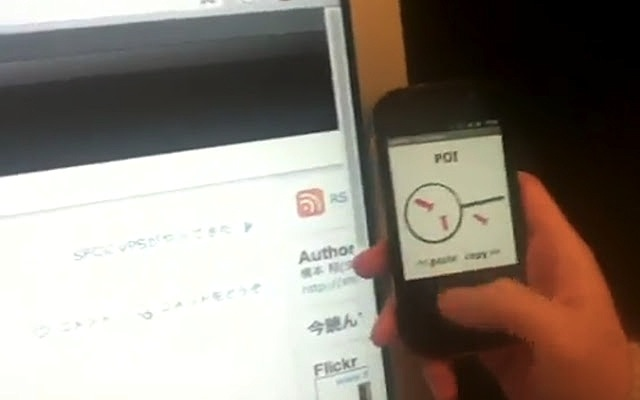
\includegraphics[height=40mm]{img/copy-paste.jpg}
  \end{center}
  \caption{実世界コピペ}
  \label{fig:copy-paste}
\end{figure}


\subsection{GoldFishフレームワークの実装}
GoldFishでは、アプリケーションの実装にAndroidネイティブのJavaではなくJavaScriptを採用している。Javaはプログラム言語自体が複雑で難しく、またセンサーの値を監視しつつ画面を更新しつつ通信も行うなどの並行処理の記述がシンプルに記述できない。JavaScriptはシンプルなプログラム言語で、初心者にもよく薦められている。そして関数がファーストクラスオブジェクトなのでタイマーを用いた並行処理の記述も容易である。

GoldFishはJavaで実装したネイティブアプリに、WebViewコンポーネントでwebページを表示している。WebView内のJavaScriptとAndroidネイティブのJavaが通信する事で、JavaScriptからセンサーなどの機能を呼び出せる。

GoldFishはNFCタグを読んだ際に、あらかじめタグに対して登録されているURLを読み込み、WebViewに表示する。NFCタグはGoldFishのwebサイトで登録できる。(図:\ref{fig:tags})
\begin{figure}
  \begin{center}
    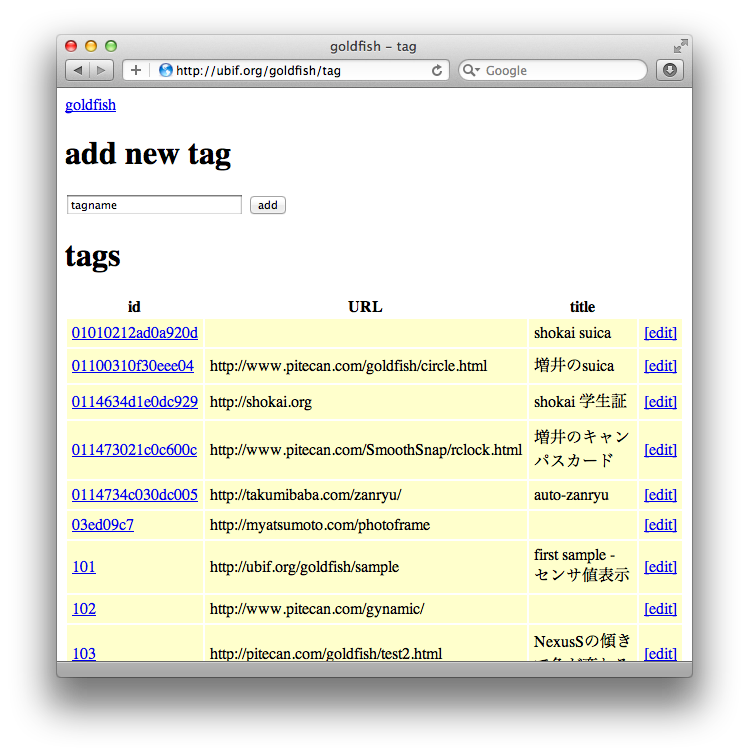
\includegraphics[height=70mm]{img/tags.png}
  \end{center}
  \caption{NFCタグ登録画面 http://ubif.org/goldfish/tag}
  \label{fig:tags}
\end{figure}

\subsection{JavaScriptによるアプリケーションの実装}
アプリケーションの実装は、GoldFishのサンプルページ\cite{sample}を見るとわかりやすい。Webページを作成し、goldfish.jsというJavaScriptライブラリを読み込むとAndroidネイティブのセンサーやGoldFish用の様々な機能が使用できる。1章で挙げた実世界GUIの実装に必要な4つの機能は、goldfish.tag関数で操作対象の指定、goldfish.gyroscopeやaccelerometerなどのセンサーによるジェスチャー入力、goldfish.id関数によるユーザーの判別、goldfish.tcpやajaxによるほかのシステムとの通信の組み合わせによって実現できる。


\section{その他のGoldFishアプリケーションの例}
前章の実世界コピペの他にも、いくつかGoldFishを用いた実世界GUIを紹介する。いずれも実装には1日かかっておらず、GoldFishを使うことで実世界GUIを簡単に素早くプロトタイピングできる事がわかる。

\subsection{ドア認証}
大学の研究室の電子錠ドアをGoldFishで開閉するシステムを実装した。(図:\ref{fig:door})Androidアプリケーション側の実装は、プログラムの基礎は学んだもののあまり書いたことのない大学3年生でも6時間ほどで実装できた。

研究室の電子錠ドアに貼ってあるNFCタグにAndroid端末で触り、ドアノブをひねるような動きでAndroid端末を回転させるとドアの鍵が開くアプリケーションである。JavaScript40行程度で書かれたGoldFishアプリケーションは、10ミリ秒毎にジャイロスコープを監視して角度が合計90度まわされるとAjaxでドアサーバーに開閉のリクエストを送る。ドアサーバーはPhidgetsサーボモーターとRubyのSinatraアプリケーションで実装されており、HTTP-POSTを受信するとドアの鍵を回して開け、5秒後に閉める。筆者らは日常的にこの仕組みを使っている。

\begin{figure}
  \begin{center}
    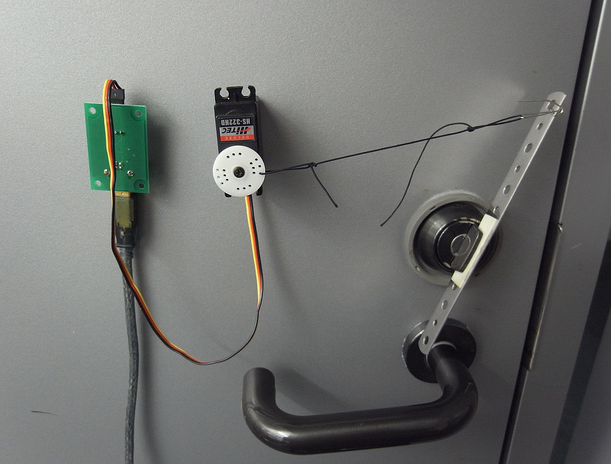
\includegraphics[height=40mm]{img/door.png}
  \end{center}
  \caption{GoldFishドアのしくみ}
  \label{fig:door}
\end{figure}


\subsection{マウス}
GoldFishのUDP/IP関数を用いて、空中で操作するマウスとトラックパッドを実装した。机にNFCタグを貼り付けておき、その上にAndroid端末を乗せると目の前のMacを操作できるトラックパッドが現れる。MacではJRubyで実装したマウスサーバーが起動しており、UDPで受信した座標にマウスを移動させたり、クリックさせたりという指示を実行できる。


\subsection{写真立て}
Android端末を机の上の写真立てに乗せると、Flickrから取得した動物の写真がスライドショーとして表示されるアプリケーションを実装した。実装にはFlickrのJavaScript APIをGoldFishのAjaxから使用した。


\section{結論}
GoldFishを使うことで実世界GUIアプリケーションを簡単に実装できる。GoldFishアプリケーションはJavaScriptで記述する事ができ、また操作対象の指定、ジェスチャーやGUIによる操作、ユーザーとコンテキストの判別、他のシステムとの通信を簡潔に記述できる機能がJavaScriptの関数として実装されている。


\begin{thebibliography}{10}

\bibitem{field-mouse}
椎尾一郎, 増井俊之, 福地健太郎. FieldMouseによる実世界指向インタフェース. コンピュータソフトウェア, Vol.18, No.1, pp. 28-38, January 2001.

\bibitem{Ubi-Finger}
塚田浩二,安村通晃: Ubi-Finger:モバイル指向ジェスチャ入力デバイスの研究, 情報処理学会論文誌, Vol.43, No.12, pp.3675-3684 (2002)

\bibitem{pick-and-drop}
Jun Rekimoto, Pick-and-Drop: A Direct Manipulation Technique for Multiple Computer Environments, Proceedings of UIST'97, pp. 31-39, 1997.

\bibitem{実世界GUI}
Toshiyuki Masui, Itiro Siio. Real-World Graphical User Interfaces. In Proceedings of the International Symposium on Handheld and Ubiquitous Computing (HUC2000), pp.72-84, September 2000. 

\bibitem{goldfish}
GoldFish. http://ubif.org

\bibitem{sample}
GoldFish App Sample. http://ubif.org/goldfish/sample

\bibitem{github}
ソースコード. https://github.com/shokai/goldfish

\end{thebibliography}

